
\documentclass[12pt]{article}
\usepackage[english]{babel}
\usepackage[utf8x]{inputenc}
\usepackage{amsmath}
\usepackage{graphicx}
\graphicspath{ {scrn/} }
\usepackage[colorinlistoftodos]{todonotes}

\begin{document}

\begin{titlepage}

\newcommand{\HRule}{\rule{\linewidth}{0.5mm}} % Defines a new command for the horizontal lines, change thickness here

\center % Center everything on the page
 
%----------------------------------------------------------------------------------------
%	HEADING SECTIONS
%----------------------------------------------------------------------------------------

\textsc{\Large UNIVERSITATEA TEHNICĂ A MOLDOVEI}\\[1cm] % Second title
\textsc{\Large Facultatea „Calculatoare, Informatică şi Microelectronică”}\\[0.5cm] % Third title
\textsc{\large Specialitatea : Tehnologii informationale}\\[0.5cm] % Minor heading 

\textsc{\large Disciplina : Medii interactive de dezvoltare a produselor soft}\\[1.5cm] % Minor heading 
\large Lucrarea de laborator nr.2\\[1cm]
%----------------------------------------------------------------------------------------
%	TITLE SECTION
%----------------------------------------------------------------------------------------

\HRule \\[0.4cm]
{ \huge \bfseries GUI development}\\[0.2cm] % Title of the document
\HRule \\[3cm]
 
%----------------------------------------------------------------------------------------
%	AUTHOR SECTION
%----------------------------------------------------------------------------------------

\begin{minipage}{0.4\textwidth}
\begin{flushleft} \large
\emph{A efectuat:}\\
\emph{}\\
\emph{A verificat:}\\
\end{flushleft}
\end{minipage}
~
\begin{minipage}{0.4\textwidth}
\begin{flushright} \large
st. gr. TI-141 \\
\textsc{Levcenco Elena}\\ % Student's Name
\textsc{ Cojanu Irina} % Teacher's Name
\end{flushright}
\end{minipage}\\[3cm]

%----------------------------------------------------------------------------------------
%	DATE SECTION
%----------------------------------------------------------------------------------------

{\large \today}\\[2cm] % Date, change the \today to a set date if you want to be precise

%----------------------------------------------------------------------------------------

\vfill % Fill the rest of the page with whitespace

\end{titlepage}
\section{Scopul lucrarii:}
Realizeaza un simplu GUI Calculator folosind  un nou IDE.
\section{Obiective:}
\begin{itemize}
\item Realizeaza un simplu GUI Calculator
\item Operatiile simple: +,-,*,/,putere,radical,InversareSemn(+/-),operatii cu numere zecimale.
\item Divizare proiectului in doua module - Interfata grafica(Modul GUI) si Modulul de baza(Core Module).
\end{itemize}
\section{Laboratory Requirements}
\label{sec:examples}

\subsection{Basic Level (nota 5 .. 6) :}
\begin{itemize}
\item Realizeaza un simplu GUI calculator care suporta functiile de baza: +, -, /, *.
\end{itemize}


\subsection{Normal Level (nota 7 .. 8):}
\begin{itemize}
\item Realizeaza un simplu GUI calculator care suporta urmatoare functii: +, -, /, *, putere, radical, InversareSemn(+/-).
\end{itemize}
\subsection{Advanced Level (nota 9 .. 10):}
\begin{itemize}
\item Realizeaza un simplu GUI calculator care suporta urmatoare functii: +, -, /, *, putere, radical, InversareSemn(+/-), operatii cu numere zecimale.
\item Divizare proiectului in doua module - Interfata grafica(Modul GUI) si Modulul de baza(Core Module).
\end{itemize}
\section{Analiza lucrarii:}
Limbaj de programare: Python\\
IDE-ul:PyCharm (JetBrains)\\
Primele pasi a crearii calculatorului constau in UI:
\begin{itemize}
\item crearea layout-ului grid
\item crearea fiecarui buton 
\item definirea fontului,background-ului,textului si functiei fiecarui buton
\end{itemize}
Functia comuna pentru toate butoane este 'btnclick',care are ca parametrul textul butonului.Functia verifica parametrul,si indeplineste instructiuni in functie de parametrul.Intructiunea principala a functiei este de evaluare a stingului obtinut prin concatenarea caracterelor la apasarea butonului.Programul prevede momente ca:
\begin{itemize}
\item impartirea la 0 este imposibila
\item un numar nu poate contine mai mult decit un punct
\item calculul '%'
\item restrictia(ex: daca utilizatorul apasa '-' si indata '+' programul rescrie operatia)
\item afisarea rezultatului float sau integer
\item afisarea operatiilor
\end{itemize}

.
Rezolvarea conflictelor:\\
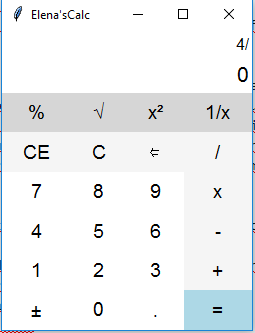
\includegraphics{divide.png}\\

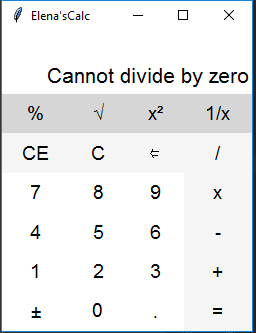
\includegraphics{0.png}\\

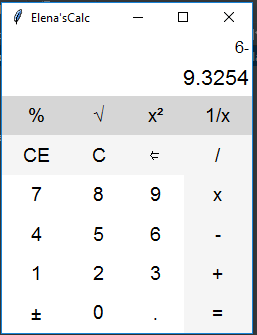
\includegraphics{decimals.png}\\

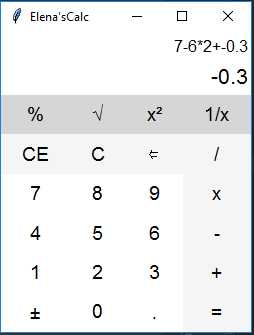
\includegraphics{example.png}\\
\section*{Concluzia}
Python este un limbaj de programare puternic si usor de învatat.Pachetul de tkinter ("interfață Tk") este interfața standard de Python pentru setul de instrumente Tk GUI. Ambele Tk și tkinter sunt disponibile pe majoritatea platformelor Unix, precum și pe sistemele de operare Windows.Laboratorul dat a constat in mare parte de instrucţiunea if care  executa o anumită porţiune de cod dacă era îndeplinită o condiţie.  
\end{document}